\documentclass{article}

\usepackage[utf8]{inputenc}
\usepackage{amsmath}
\usepackage{amssymb}
\usepackage{anysize}
\usepackage{color}
\usepackage{xcolor}
\usepackage{graphicx}
\usepackage{float}

\usepackage{subfigure}

\definecolor{dkgreen}{rgb}{0, 0.6, 0}
\definecolor{gray}{rgb}{0.5, 0.5, 0.5}
\usepackage{listings}
%\lstset{language=Matlab,
%   keywords={break,case,catch,continue,else,elseif,end,for,function,
%      global,if,otherwise,persistent,return,switch,try,while},
%   basicstyle=\ttfamily,
%   keywordstyle=\color{blue},
%   commentstyle=\color{red},
%   stringstyle=\color{dkgreen},
%   numbers=left,
%   numberstyle=\tiny\color{gray},
%   stepnumber=1,
%   numbersep=10pt,
%   backgroundcolor=\color{white},
%   tabsize=4,
%   showspaces = false,
%   showstringspaces = false}
\lstset{
	language=Matlab,                	% choose the language of the code
	keywords={break,case,catch,continue,else,elseif,end,for,function,
      global,if,otherwise,persistent,return,switch,try,while},
      keywordstyle=\color{blue},
      commentstyle=\color{red},
	basicstyle=\footnotesize,       % the size of the fonts that are used for the code
	numbers= left,                 	% where to put the line-numbers
	numberstyle=\footnotesize,      % the size of the fonts that are used for the line-numbers
	stepnumber=1,                   % the step between two line-numbers. If it is 1 each line will be numbered
	numbersep=5pt,                  % how far the line-numbers are from the code
	backgroundcolor=\color{white},  % choose the background color. You must add \usepackage{color}
	showspaces=false,               % show spaces adding particular underscores
	showstringspaces=false,         % underline spaces within strings
	showtabs=false,                 % show tabs within strings adding particular underscores
	frame=single,           		% adds a frame around the code
	tabsize=2,          			% sets default tabsize to 2 spaces
	captionpos=t,          			% sets the caption-position to bottom (t=top, b=bottom)
	breaklines=true,        		% sets automatic line breaking
	breakatwhitespace=false,    	% sets if automatic breaks should only happen at whitespace
	escapeinside={\%*}{*),  % if you want to add a comment within your code
	flexiblecolumns=true}         
}

%\lstset{
%	language=Matlab,                	% choose the language of the code
%	basicstyle=\footnotesize,       % the size of the fonts that are used for the code
%	numbers= left,                 	% where to put the line-numbers
%	numberstyle=\footnotesize,      % the size of the fonts that are used for the line-numbers
%	stepnumber=1,                   % the step between two line-numbers. If it is 1 each line will be numbered
%	numbersep=5pt,                  % how far the line-numbers are from the code
%	backgroundcolor=\color{white},  % choose the background color. You must add \usepackage{color}
%	showspaces=false,               % show spaces adding particular underscores
%	showstringspaces=false,         % underline spaces within strings
%	showtabs=false,                 % show tabs within strings adding particular underscores
%	frame=single,           		% adds a frame around the code
%	tabsize=2,          			% sets default tabsize to 2 spaces
%	captionpos=t,          			% sets the caption-position to bottom (t=top, b=bottom)
%	breaklines=true,        		% sets automatic line breaking
%	breakatwhitespace=false,    	% sets if automatic breaks should only happen at whitespace
%	escapeinside={\%*}{*),  % if you want to add a comment within your code
%	flexiblecolumns=true}         
%}

\usepackage{caption}
\DeclareCaptionFont{white}{\color{white}}
\DeclareCaptionFormat{listing}{\colorbox{gray}{\parbox[c]{\textwidth}{#1#2#3}}}
\captionsetup[lstlisting]{format=listing,labelfont=white,textfont=white}

\setlength\parindent{0pt}
\setlength{\parskip}{10pt}

\marginsize{3cm}{2cm}{2cm}{2cm}

\title{Autonomous Robotics\\
		Wavefront Planner\\
		Lab 1 Report}
\author{Emre Ozan Alkan\\
		\{emreozanalkan@gmail.com\}\\
		MSCV-5}
\date{\today}

\begin{document}
\maketitle

\section{Introduction}

	Path planning is very important in robotics. Also finding optimal trajectory is hard and highly demanded task in autonomous robotics. In this lab, we implemented path planning algorithm, based on potential functions, called ''Wavefront Planner'' to solve simple path plannig problem in Matlab.

	\subsection{Environment}
	
	In this lab, we had two 2D environment. In these environments; obstacles, empty spaces and goal position are marked as 1, 0 and 2 respectively. We had to find optimal trajectory way between given start position and the goal position marked as 2.

\begin{figure}[ht!]
\begin{center}
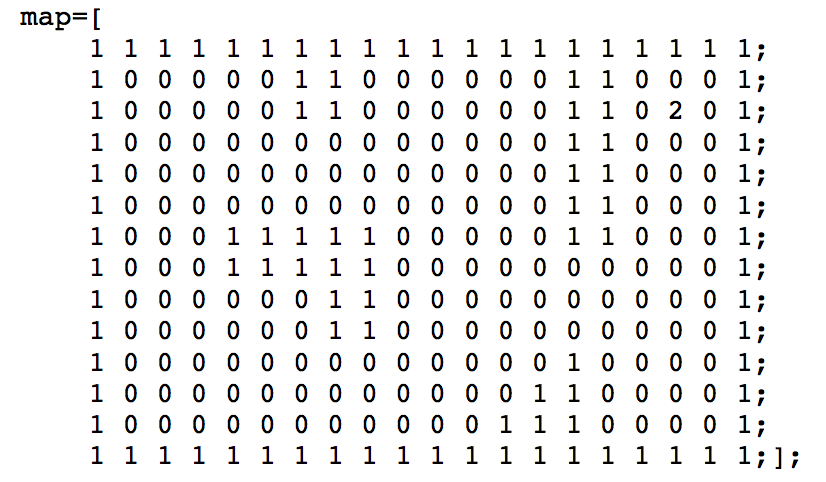
\includegraphics[scale=0.4]{mapMatrix.png}
\caption{20x14 Sample Environment}
\end{center}
\end{figure}
	
	\subsection{Wavefront Planner}
	Wavefront Planner consist of creating potential map from given start point and finding optimal trajectory between the given start point and the marked goal position. So in this lab, we implemented Wavefront Planner in 2 part; first building potential map and then finding optimal trajectory. My implementation considering 8-point connectivity for better optimal results, but able to easily switch 4-point connectivity.
	
\begin{figure}[ht!]
\centering
\subfigure[20x14 Environment]{
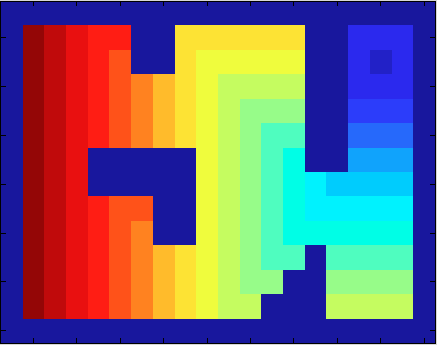
\includegraphics[width=.380\textwidth]{potentialMap1.png}
}
\subfigure[242x242 Environment]{
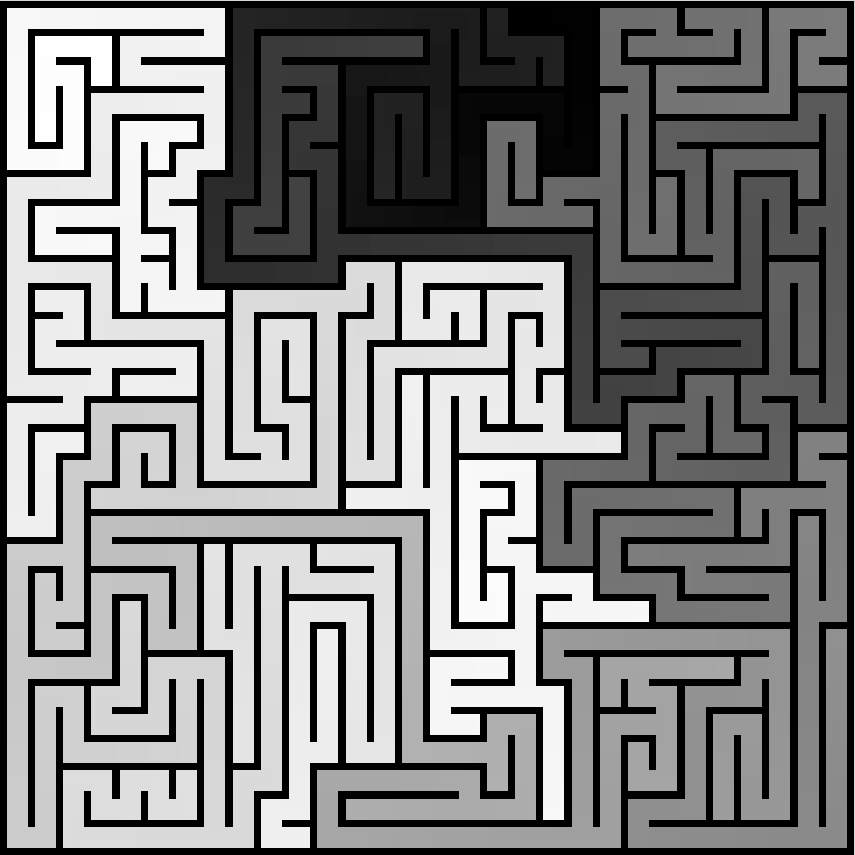
\includegraphics[width=.300\textwidth]{potentialMap2.png}
}
\caption{Sample Potential Maps}
%\label{fig:whatever}
\end{figure}

\section{Implementation}

	In Matlab implementation, I've found difficulties and encountered with problems.Also I've made a mistake by testing and building my implementation with first 20x14 environment which caused failure in bigger and complex environments. \par
	While implementing my optimal trajectory finding, firstly I assumed that moving diagonal is not costly but changing direction is costly for robot. Secondly, I wanted to store previous direction(4-connectivity or 8-connectivity move) so that If previous move was on diagonal and if there 2 or more optimal path, I added euclidean distance check with candidate points and goal position to pick optimal move which has minimal euclidean distance. By this I thought robot will make less direction change, but this approached failed on more detailed and complex maps. So I had to turn off robot direction and euclidean distance check to get expected results.

	\subsection{Problems and Difficulties}
	
		\subsubsection{Finding Optimal Path}	
		
		In our lab paper, under 2. section "Wavefront Planner", there is an image(Figure 3 below) showing one of the best optimal trajectory. It is going straight, making diagonal turn, keep going till coming straight under the goal, making turn and going the goal directly.
		
\begin{figure}[ht!]
\begin{center}
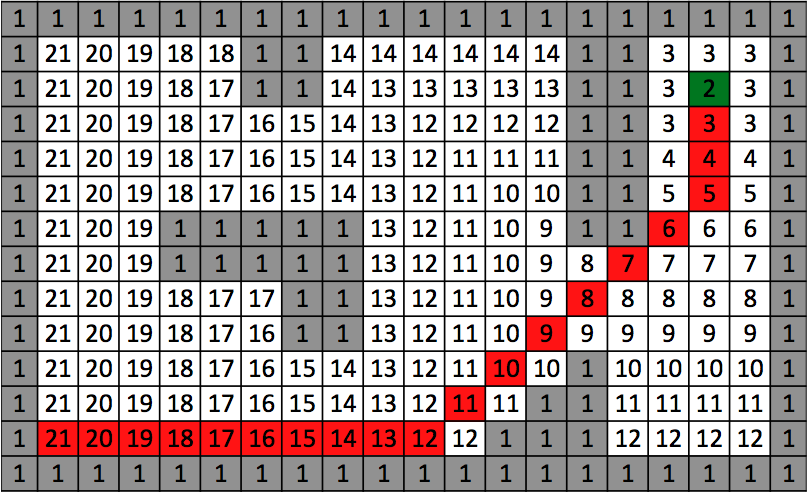
\includegraphics[scale=0.1]{optimalTrajectory1.png}
\caption{20x14 Sample Environment with Optimal Trajetory}
\end{center}
\end{figure}

	I also wanted to implement my Warefront Planner in a same way that optimizing robot direction changes minimized, because in the lab paper under representation part, and in our algorithm, we find a trajectory that it requires another diagonal turn near goal.
	
	In order to solve this problem, we were discussing the problem with my friend Devesh, and we found that, what if we keeping inertial momentum of the robot, if it is going straight or diagonal we would force it to keep its direction. However this approach was failing and producing more diagonal turns. Later I added another constraint to consider which is if robot's previous move was diagonal, I was checking euclidean distance between optimal candidates and the goal which worked fine in our 14x20 environment. However this approach is failed, and I've turned off this approach in implementation, and got expected results.
	
\begin{figure}[ht!]
\begin{center}
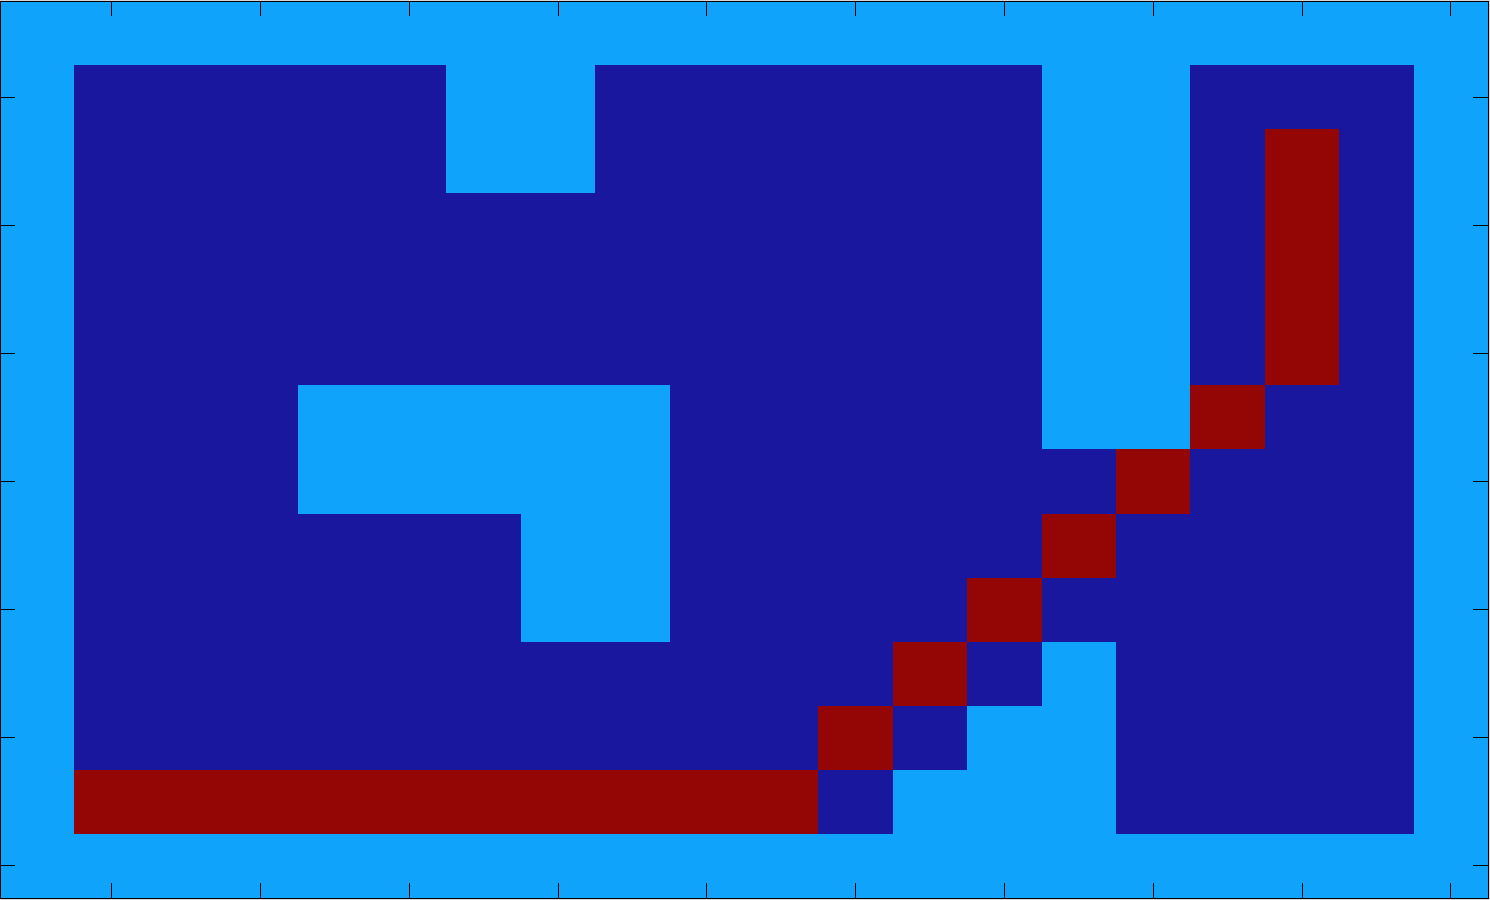
\includegraphics[scale=0.1]{optimalTrajectory2.png}
\caption{20x14 Sample Environment with Optimal Trajectory created by My Algorithm}
\end{center}
\end{figure}

		\subsubsection{Matlab Limitations}
		
		 Having good programming skills in C++, Java, CSharp weren't helping me much when programming in Matlab where I'm not good at. While building potential map(value map in implementation) for Wavefront Planner, we needed queue or some list to store neighbors to visit and give them a value. I would use classic Matlab matrices, however changing size in each iteration adding to bottom and removing each time from top didn't seem optimal to me. So after searching, I found that we are able to use Java in Matlab, where we can just import java.util and use it's classes. However it was limited that we can't provide Comparer for sorting the list. Whereas for building trajectory, I had to sort some rows according to their values or euclidean distances, so I decided to use Matlab matrices in trajectory building to use sortrows() functionality. \par
		  Another limitation is Matlab doesn't support pass by reference for its built in types. So whenever I pass argument to function and change in in function, I had to return the changed one back. Hence I used lots of parameters and return parameters which slowed my implementation. \par
		  Since coming from strong object oriented programming background, I didn't want to use global variables which I dislike a lot, so everything was local. I really wanted to create "WavefrontPlanner" Matlab class to wrap all logic to program this lab with object oriented design however this lab was limited with sending only 1 implementation file and 1 report. So I had troubles in Matlab programming a lot.

	\subsection{Functions}
	My implementation consist of 4 main functions; 'wavefront' - main function to call, 'buildValueMap' - building value map/potential map, 'buildTrajectory' - building optimal trajectory, 'displayWavefront' - displaying the result with given map and found trajectory. \par
	Beside this functions, many helper functions are implemented to support my algorithm. Here are short preview to my wavefront.m file with function:
	
	\begin{lstlisting}[label=wavefront-m, caption=wavefront.m]
	
function [value_map, trajectory] = wavefront(map, start_row, start_column)
%WAVEFRONT Planner algorithm to compute the optimal path towards the goal
%   Uses 8-point connectivity.

    MAP_GOAL_VALUE = 2; % GOAL VALUE SET TO: 2
    
    value_map = buildValueMap(map, MAP_GOAL_VALUE);
    
    trajectory = buildTrajectory(value_map, start_row, start_column, MAP_GOAL_VALUE);
    
    displayWavefront(map, trajectory);

end

% Displaying result with raw map and found trajectory
function displayWavefront(map, trajectory)
...    
end

%% BUILD WAVEFRONT VALUE MAP FUNCTIONS

% Building value map / potential map
function value_map = buildValueMap(map, goalValue)

    tic;

    [goalX, goalY] = findValueMapGoalPosition(map, goalValue);

    import java.util.ArrayDeque
    neighborList = ArrayDeque();

    % initiating 8-neighbor list
    map = add8NeighborToList(neighborList, goalX, goalY, goalValue, map);
    while ~neighborList.isEmpty()
        neighborData = neighborList.pop(); % or poll(), removeFirst(), remove(), pollFirst()
        % neighborData(1): x coordinate
        % neighborData(2): y coordinate
        % neighborData(3): value of cell who added this cell as neighbor
        map = add8NeighborToList(neighborList, neighborData(1), neighborData(2), neighborData(3), map);
    end
    
    value_map = map;
    
    display('Building Value Map Finished:');
    
    toc;
    
end

% finding the goal position in map
function [goalX, goalY] = findValueMapGoalPosition(map, goalValue)
...
end

% adding the 4 neighbor to list
function [changedMap] = add4NeighborToList(neighborList, x, y, currentValue, map)
...
end

% adding the 8 neighbor to list
function [changedMap] = add8NeighborToList(neighborList, x, y, currentValue, map)
...
end

% checking neighbor against overflows, and adding given neighbor to list
function [changedMap] = addNeighborToList(neighborList, neighborX, neighborY, currentValue, map)
...
end

%% BUILD TRAJECTORY FUNCTIONS

% building optimal trajectory with given value map/potential map
function [trajectory] = buildTrajectory(value_map, start_row, start_column, goalValue)

    tic;
    
    [goalX, goalY] = findValueMapGoalPosition(value_map, goalValue);
    
    robotDirection = 0; % Robot's Current Momentum Direction STRAIGHT: 0, DIAGONAL: 1
    
    trajectory = [start_row start_column]; % sortrows(matrix, column);
    
    neighborList = getAvailable8NeighborList(value_map, start_row, start_column); % init starting
    
    while ~isReachedGoal(neighborList, goalValue)
        
        [neighborX, neighborY, robotDirection] = pickNextOptimalNeighbor(neighborList, robotDirection, goalX, goalY);
        
        trajectory = [trajectory; [neighborX, neighborY]];
        
        neighborList = getAvailable8NeighborList(value_map, neighborX, neighborY);
        
    end
    
    trajectory = finalizeTrajectoryWithGoal(trajectory, neighborList);
    
    display('Building Trajectory Finished:');
    
    toc;
    
end

% checking neighbor if avaliable and optimal and If neighbor is in map borders and lower value
function [isNeighborAvailableAndOptimal] = isNeighborAvailableAndOptimal(value_map, x, y, currentValue)
...
end

% getting neighbor data, neighbor's x, y, neighbor value and if it is diagonal or not
function [neighborData] = getNeighborData(value_map, x, y, robotDirection)
...
end

% gets available 4-connectivity neighbor list of given x, y
function [neighborList] = getAvailable4NeighborList(value_map, x, y)
...
end

% gets available 8-connectivity neighbor list of given x, y
function [neighborList] = getAvailable8NeighborList(value_map, x, y)
...
end

% Checking if robot reached goal. Check is based on checking neighbors if contains goal value
function [isReachedGoal] = isReachedGoal(neighborList, goalValue)
...
end

% If robot reached goal, we adding trajectory list the goal's position.
function [trajectory] = finalizeTrajectoryWithGoal(trajectory, neighborList)
...
end

% Where next neighbor picking decision made for trajectory building.
function [neighborX, neighborY, robotDirection] = pickNextOptimalNeighbor(neighborList, robotDirection, goalX, goalY)
...
end

	\end{lstlisting}

\section{Results}

	\subsection{Representation}
	
	After finding the potential/value map and trajectory, we display the result as:
	
\begin{figure}[ht!]
\centering
\subfigure[20x14 Environment]{
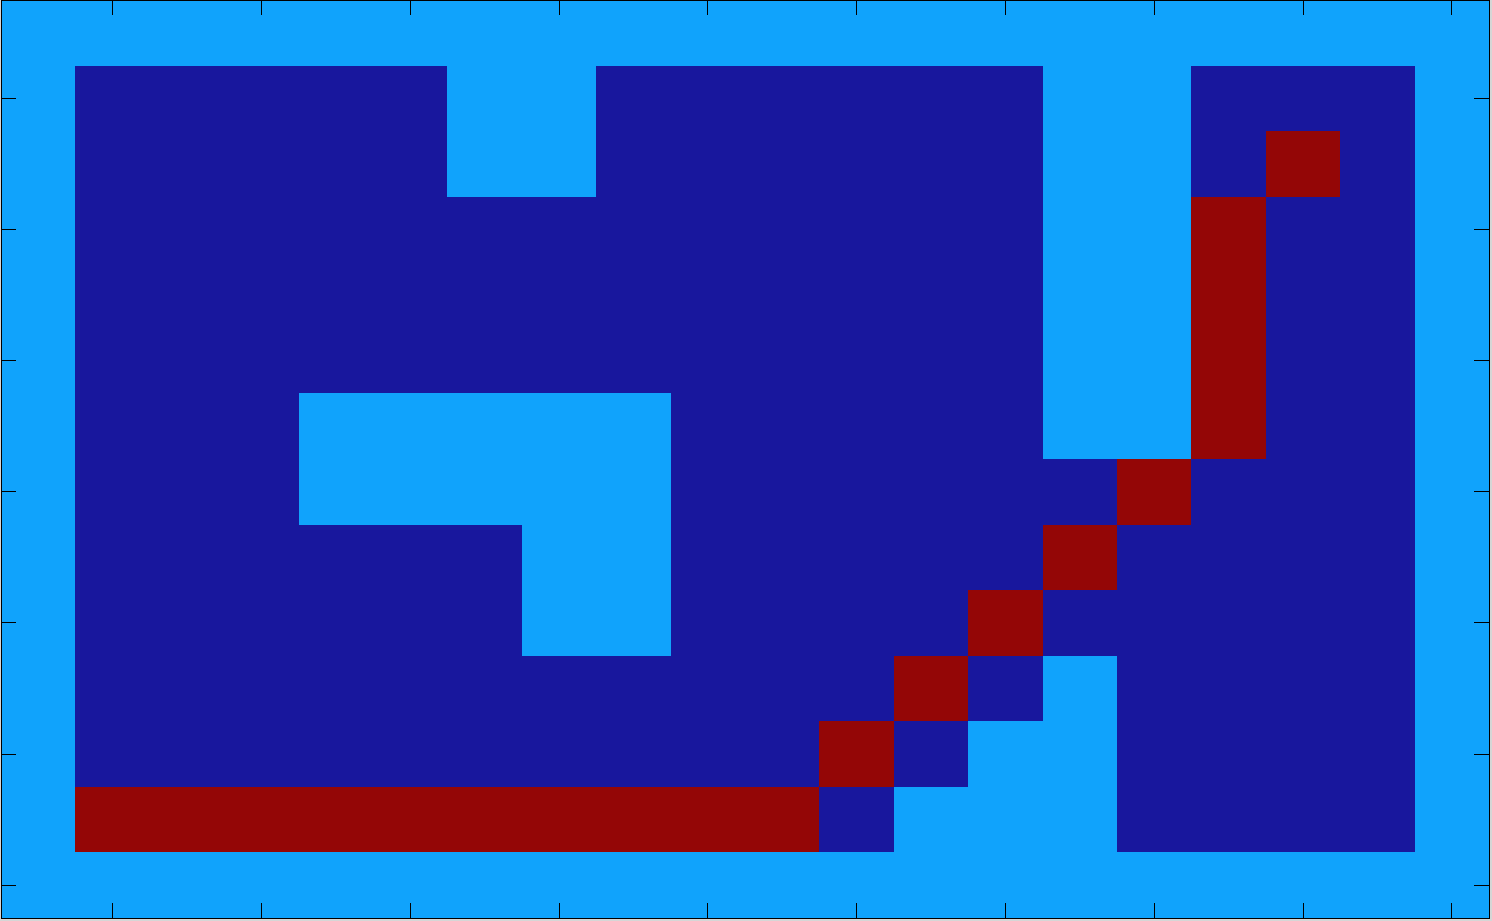
\includegraphics[width=.400\textwidth]{result1.png}
}
\subfigure[242x242 Environment]{
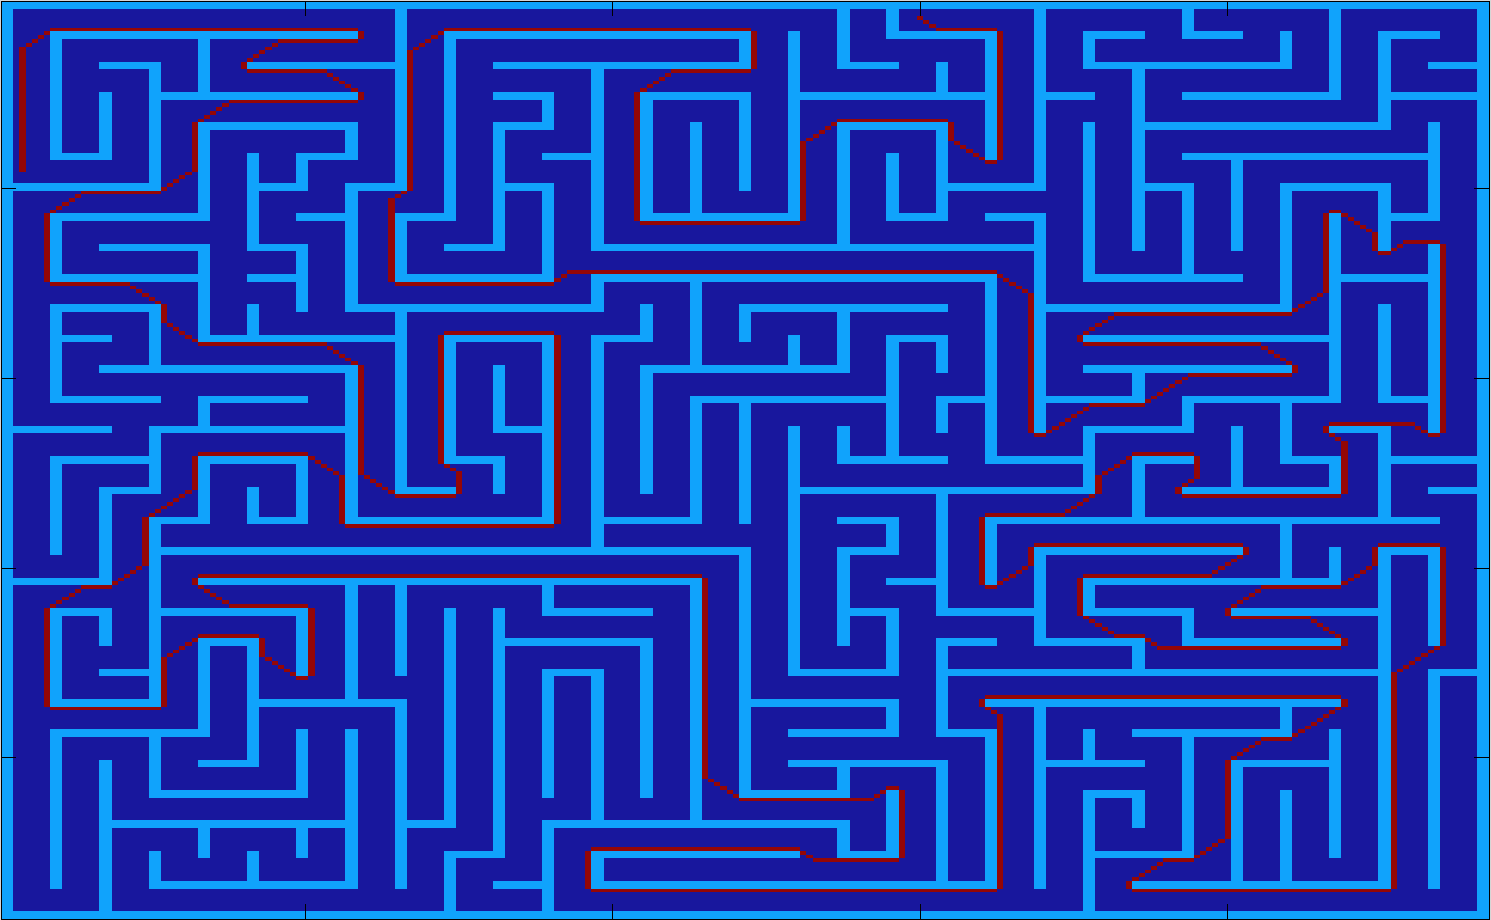
\includegraphics[width=.900\textwidth]{result2.png}
}
\caption{Wavefront Planner Results}
%\label{fig:whatever}
\end{figure}
	
	
	\subsection{Failure}
	This part of the report is for my failed approach which was keeping robot's previous direction and if previous move was diagonal, checking euclidean distance between optimal neighbors and the goal. However even this approached worked well for first environment, it failed on second environment. Here is the results with robot direction checking enabled.
	
\begin{figure}[ht!]
\begin{center}
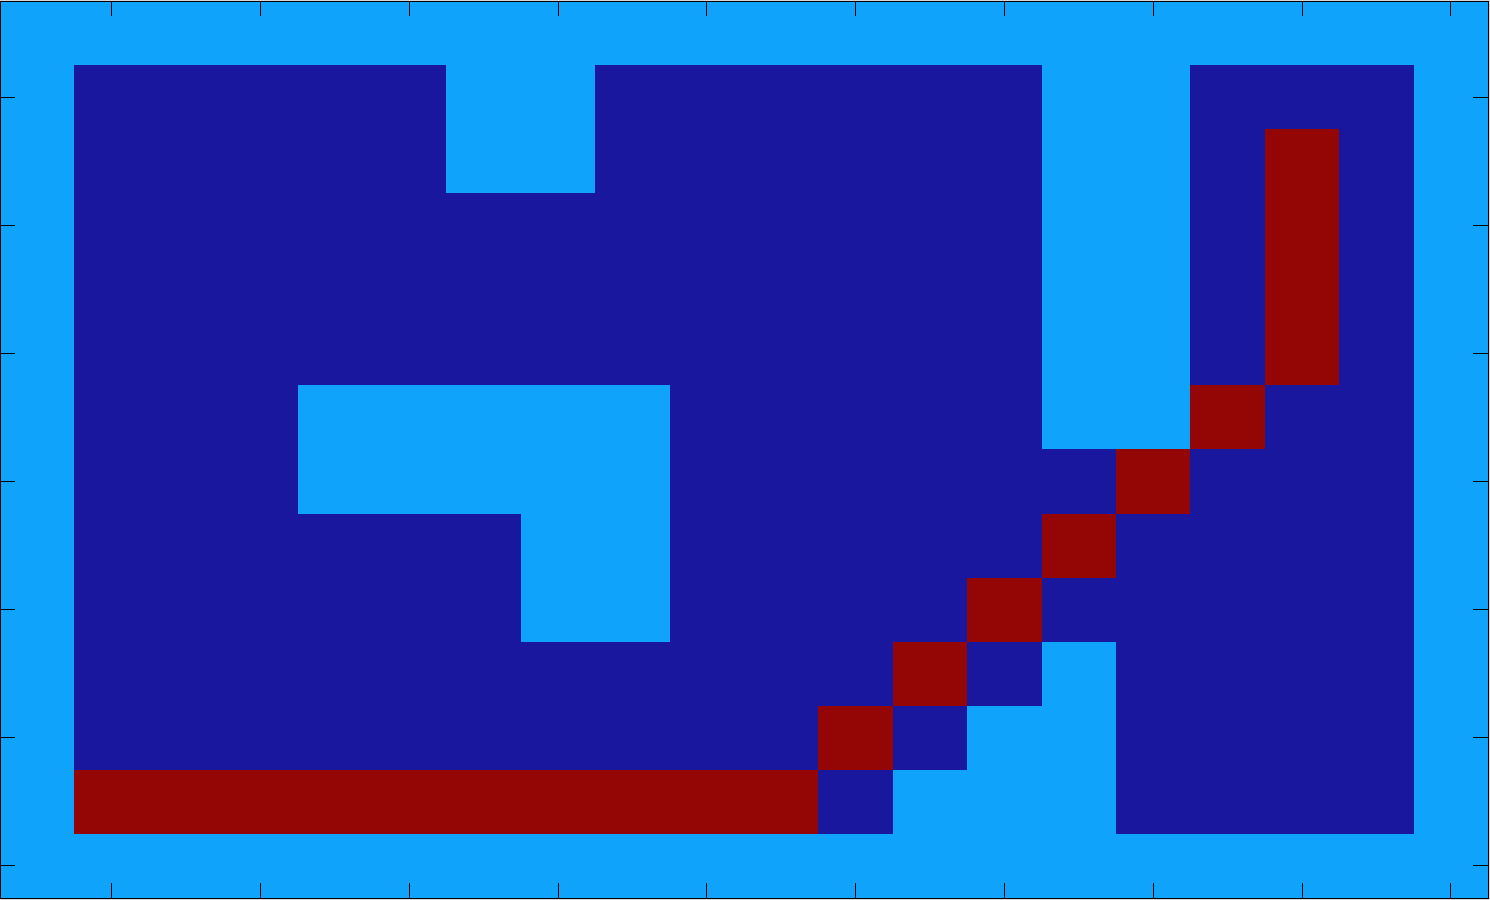
\includegraphics[scale=0.1]{optimalTrajectory2.png}
\caption{20x14 Sample Environment with Optimal Trajectory created by My Failed Algorithm}
\end{center}
\end{figure}

\begin{figure}[ht!]
\begin{center}
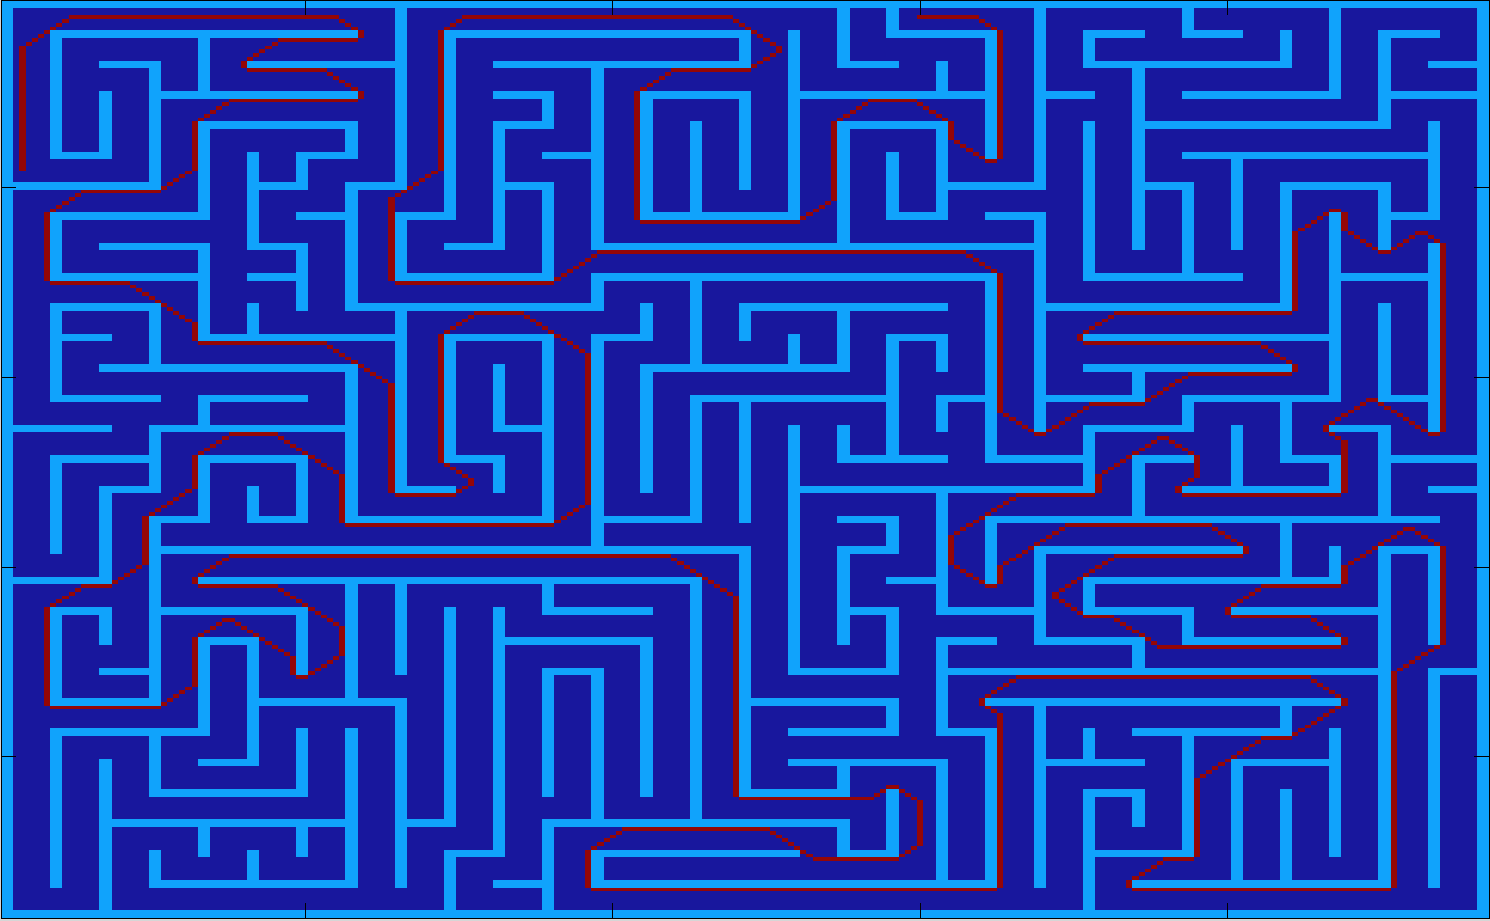
\includegraphics[scale=0.32]{failedResult1.png}
\caption{242x242 Sample Environment with Not Optimal Trajectory created by My Failed Algorithm}
\end{center}
\end{figure}


\end{document}







































